\chapter{Casos de estudio}

Ya hemos presentado el verificador de modelos MC2 y el lenguaje de descripción asociado al mismo. Es hora de observar algunos ejemplos concretos de uso de esta herramienta, y ese es el propósito de este capítulo final. Veremos como modelar tres clásicos juegos solitarios de lógica y estrategia, y analizaremos hasta que punto es viable describir manualmente el modelo con esta versión de MC2.

\section{Cruce del río}

Existen muchas versiones de este problema, nosotros modelaremos una de las versiones mas conocidas \cite{Hadley:12}. El problema es el siguiente, un granjero va a comprar un zorro, un ganso y una bolsa de frijoles. Mientras vuelve a su casa, se encuentra con que debe cruzar un río, para lo cual alquila un bote. El granjero solo puede llevar una de sus compras en el barco. Si se deja al zorro con el ganso, el zorro se lo va a comer, y si se deja al ganso con la bolsa de frijoles, este se va a comer los frijoles. El desafío del granjero es el de llevar todas sus compras intactas al otro lado del río. El problema consiste entonces en elegir sabiamente que compras trasladar en cada viaje.\\
\\
La descripción MC2 para el modelo de este problema esta en la figura \ref{fig:river}. Para modelarlo declaramos tres pares de proposiciones atómicas, uno para cada compra ($f$ representa los frijoles,$z$ el zorro y $g$ el ganso), las proposiciones marcadas con $1$ hacen referencia a que están del lado $origen$ del río, y las marcadas con $2$ hacen referencia a que están del lado $destino$ del río. Luego declaramos la variable proposicional $boat$ que si es verdadera representa al bote del lado $origen$ y en caso contrarío estará del lado $destino$. Por último declaramos $go$ que sirve para que el granjero no pueda viajar hasta que no pase algo del otro lado del río. En cuanto a las reglas, hay dos grupos de reglas a tener en cuenta para describir el comportamiento del sistema, por un lado se describe lo que pasa cuando se dejan juntos objetos (si son incompatibles, uno es comido, sino, no pasa nada), por otro lado tenemos las reglas que definen la acción de viajar de un lado del río al otro (se puede viajar solo o acompañado por un solo objeto). Hay que destacar que, por ejemplo, si $f1$ y $f2$ son falsas significa que los frijoles se han comido, y ninguna regla puede cambiar estos valores. En este caso, en el estado inicial queremos que valga que tanto el granjero/bote como el zorro, el ganso y los frijoles están del lado $origen$ del río. Por último, la propiedad que queremos verificar es si es alcanzable un estado donde, siguiendo las reglas, puedan estar el zorro, el ganso y los frijoles en el lado $destino$ del río.

\begin{figure}[H]
  \centering
  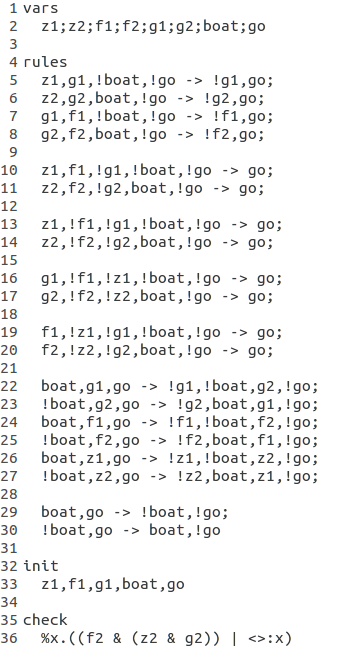
\includegraphics[width=0.6\textwidth]{Figures/rivercross.png}
  \caption{Descripción de modelo del problema del cruce del río.}
  \label{fig:river}
\end{figure}

\section{1,2,3, Coloca otra vez}

Se parte de una estrella de 5 puntas, ademas de estas, se forman 5 puntos en su interior. Partiendo de uno de los 10 puntos donde no haya una ficha previamente colocada, se cuenta tres posiciones consecutivas sobre una de las aristas que contienen el punto de partida. Tras ello, se coloca una ficha en la tercera posición. En la figura \ref{fig:pentagrama} podemos ver la estrella, hemos nombrado los puntos externos como $o1, ..., o5$ y los internos como $i1, ..., i5$. Por ejemplo partiendo de $o1$ podemos poner una ficha en $i3$ o $i5$. El conteo puede pasar por una posición en la que haya ficha, pero no puede iniciarse en una posición con ficha. El juego estará resuelto cuando se hayan colocado 9 fichas \cite{Juegos:11}. 

\begin{figure}[H]
  \centering
  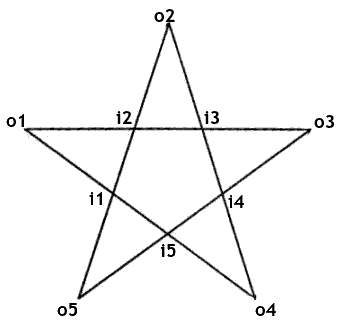
\includegraphics[width=0.5\textwidth]{Figures/pentagram.png}
  \caption{Pentagrama de 1,2,3 Coloca otra vez.}
  \label{fig:pentagrama}
\end{figure}

\noindent En la figura \ref{fig:estrella} se puede ver la descripción MC2 para el modelo de este problema. Para este modelo, declaramos una proposición para cada uno de los diez puntos de la estrella, donde cada proposición es verdadera o falsa dependiendo de si hay o no una ficha en ese punto. Las reglas en este caso representan las jugadas posibles a partir de cada punto. En el estado inicial no hace falta describir nada, ya que inicialmente queremos que no haya ficha en ningún punto de la estrella (todas las proposiciones están inicializadas en $False$). Por último, la propiedad que queremos verificar es si es posible poner nueve fichas en la estrella, a modo de ejemplo, la formula pide que haya una ficha en todos los puntos excepto $i5$.

\begin{figure}[H]
  \centering
  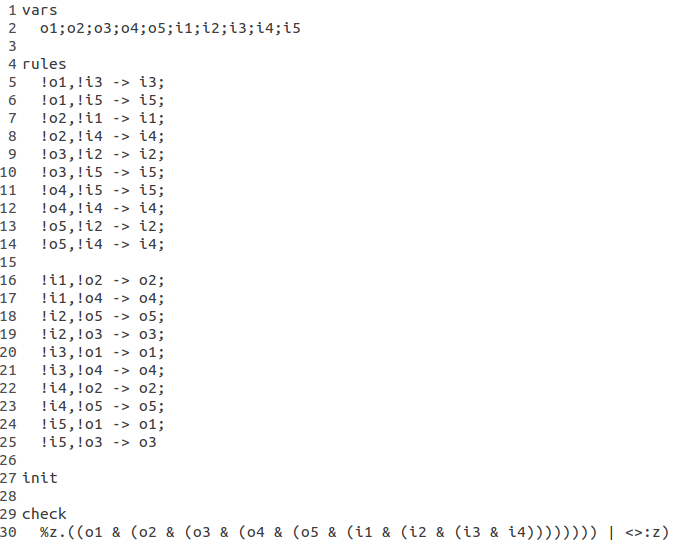
\includegraphics[width=1\textwidth]{Figures/estrella.png}
  \caption{Descripción de modelo del problema de 1,2,3 Coloca otra vez.}
  \label{fig:estrella}
\end{figure}

\section{Ranas saltarinas}

En este juego se tiene una tira de papel dividida en siete casillas \cite{Juegos:11}. La posición inicial es la indicada con tres fichas azules (blancas) y tres rojas (grises) colocadas como en la figura \ref{fig:ranasjuego}. El objetivo del juego consiste en permutar las posiciones de las fichas azules y rojas. Es decir, las azules han de pasar a ocupar las posiciones de las rojas y viceversa. Para ello son válidos los siguientes movimientos:\\
\\
- Una ficha puede moverse a un lugar contiguo, si éste está vacío.\\
\\
- Una ficha junto a otra de distinto color puede saltar por encima de ella si el salto (por encima de una sola ficha) le lleva a una casilla vacía.\\
\\
- Son válidos tanto los movimientos hacia atrás como hacia adelante.\\
\\

\begin{figure}[H]
  \centering
  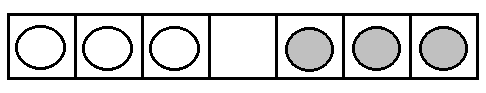
\includegraphics[width=0.8\textwidth]{Figures/ranasjuego.png}
  \caption{Juego de las ranas saltarinas.}
  \label{fig:ranasjuego}
\end{figure}

\noindent La descripción MC2 del modelo para este juego esta en la figura \ref{fig:ranas}. En este caso, tenemos siete proposiciones que representan la ocupación de cada casilla por una ficha roja, y siete más para las fichas azules, es de imaginar que una casilla $i$ esta vacía si $ri$ y $bi$ son falsas, donde $ri$ significa que hay una ficha roja en la i-ésima casilla, y $bi$ significa que hay una azul en la misma casilla. Las reglas están divididas en cuatro bloques, dos para cada dirección en la que se puede mover una ficha. Los dos bloques de una dirección representan las primeras dos reglas del juego. Por su puesto, los bloques de la otra dirección son análogos. Como estado inicial tenemos las fichas azules colocadas del lado izquierdo de la tira de casillas, y las rojas del lado derecho, dejando vacía la casilla del medio. Por último, una propiedad interesante que podemos verificar es si es posible permutar las posiciones de las fichas rojas con las azules y viceversa, desde todos los estados alcanzables por el inicial. 

\begin{figure}[H]
  \centering
  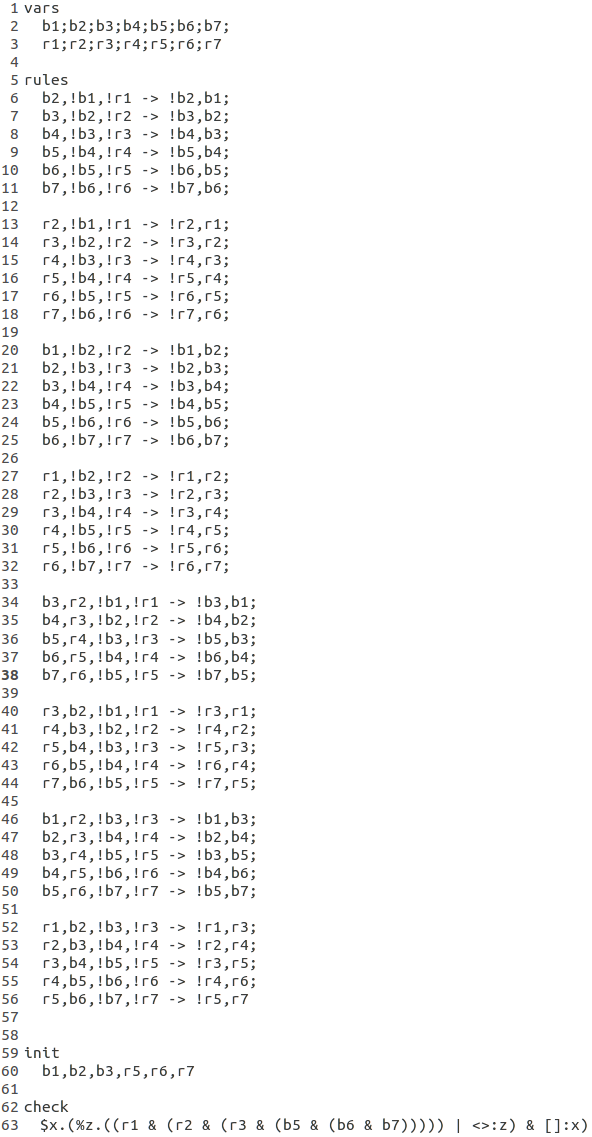
\includegraphics[width=0.6\textwidth]{Figures/ranas.png}
  \caption{Descripción de modelo del problema de las ranas saltarinas.}
  \label{fig:ranas}
\end{figure}

\noindent Nos podemos preguntar como sería la descripción MC2 del modelo si la tira tuviera más de siete casillas, esta claro que cada vez se vuelve más humanamente inviable a medida que se incrementa el tamaño de casillas. Esto es debido a que la herramienta no cuenta actualmente con abstracciones estructurales como los arreglos. Pero no es difícil escribir un programa en un lenguaje de alto nivel que genere una descripción MC2 para un sistema determinado, por ejemplo, para generar el modelo del problema de las ranas saltarinas pero con $N$ casillas.

\chapter*{Conclusión}
\addcontentsline{toc}{chapter}{Conclusión}

Para el desarrollo de esta tesis, se ha investigado sobre la verificación de modelos, sus variantes como la verificación de modelos explícitos y la verificación de modelos simbólicos, para lo cual también fue necesario investigar sobre lógicas temporales para llegar así a entender el {\mucalculo} y aplicarlo a la práctica.\\
\\
Se logró desarrollar una nueva herramienta de verificación de modelos para {\mucalculo}, con un lenguaje de modelado propio basado que permite describir de manera intuitiva diversos tipos de sistemas, entre ellos, acertijos lógicos. Mediante el model checker se puede determinar si el modelo cumple con las propiedades deseadas por el usuario (en el caso de un acertijo, determinar si hay solución por ejemplo). Se puede destacar que existen algunas herramientas de model checking para {\mucalculo} como mCRL2 \cite{Groote:14}, TAPAs \cite{Calzolai:15} y CWB \cite{Moller:13}. Sin embargo, ninguna de estas está implementada en lenguajes funcionales, una implementación funcional posee algunas ventajas, por ejemplo la simplicidad al verificar correctitud y la transparencia de las definiciones.\\
\\
Como trabajos futuros, se puede considerar la idea de hacer más versátil el lenguaje de modelado, ya sea agregando más tipos de datos y/o extendiendo las formas de expresar el flujo del sistema que se está modelando. Además como el foco de atención en el desarrollo de la herramienta no fue la eficiencia, se puede mejorar notoriamente en este aspecto.